\documentclass[]{scrartcl}

\title{\LARGE \color{darkgreen}Radio K.A.O.S\color{black}: 
              Cognitive Radio with Dynamic Spectrum Sharing Engine}
\subtitle{\vspace{3ex} \Large Project Proposal Document}
\author{
    \large \textit{Omar Eltobgy} (41)\hspace{5ex}
    \large \textit{Mohamed Elmansour} (55)\hspace{5ex}
    \large \textit{Mostafa Abd El-Aziz} (67)\\
}
\date{\large \today}

% font
\usepackage[T1]{fontenc}
\usepackage{lmodern}
\usepackage{sfmath}
\usepackage{microtype}
\usepackage[utf8]{inputenc}
% \usepackage{cfr-lm} % font package

% listings
\usepackage{listings}
\usepackage{color}
\definecolor{mygreen}{rgb}{0,0.6,0}
\definecolor{mygray}{rgb}{0.5,0.5,0.5}
\definecolor{mymauve}{rgb}{0.58,0,0.82}
\lstset{ %
  backgroundcolor=\color{white},
  basicstyle=\footnotesize\ttfamily,
  breakatwhitespace=false,
  breaklines=true,
  captionpos=b,
  commentstyle=\color{mygreen},
  deletekeywords={...},
  escapeinside={\%*}{*)},
  extendedchars=true,
  frame=single,
  keepspaces=true,
  keywordstyle=\color{blue},
  language=r,
  otherkeywords={*,...},
  numbers=none,
  numbersep=5pt,
  numberstyle=\tiny\color{mygray},
  rulecolor=\color{black},
  showspaces=false,
  showstringspaces=false,
  showtabs=false,
  stepnumber=2,
  stringstyle=\color{mymauve},
  tabsize=2,
  title=\lstname
}

% margins
\usepackage[margin=3cm,a4paper]{geometry}

% figures and tables
\usepackage{graphicx}
\usepackage{float}

% table of contents
\usepackage{tocloft}
\renewcommand{\cftsecleader}{\cftdotfill{\cftdotsep}} % for chapters
\renewcommand{\cftpartleader}{\cftdotfill{\cftdotsep}} % for parts

% section style
\usepackage{sectsty}
\sectionfont{\LARGE}

% page orientation
\usepackage{lscape}

% hyperlinks
\usepackage{hyperref}

% colors
\definecolor{darkgreen}{RGB}{0, 100, 0}

%------------------------------------------------------------------------------%

\begin{document}

% university logo
\titlehead{

    \small Alexandria University\\
    \small Faculty of Engineering\\
    \small Computer and Systems Engineering Department\\
    \small CS 436 - Topics in Computer Networks

    \vspace{-2.2cm}
    \hfill
    
\includegraphics[scale=0.6]{logo.png}
}

% document title
\maketitle

%------------------------------------------------------------------------------%

\section{Abstract}

In this document we propose an idea for Wireless Networking course project. The
proposed project is basically an implementation for a cognitive radio network 
system. The system mainly consists of two parts: software-defined radio (SDR)
and cognitive engine (CE). The SDR is to be implemented on FPGA (or ASIC, 
depends on the availability of resources), while the cognitive engine will
be written in software. We chose the problem of dynamic spectrum sharing
to be the main concern of the CE.

\section{Introduction}

It's clear that this era has witnessed great advance in wireless technology.
However, the utilization of the electromagnetic spectrum is still not 
efficient due to static allocation of the spectrum. That's why research has
been done that addresses the concept of dynamic spectrum allocation to make
use of spectrum holes. \\

\begin{figure}[H]
\begin{center}
  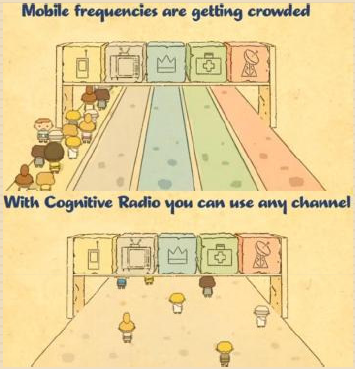
\includegraphics[scale=0.5]{cognitive1.png}
  \caption{Cognitive Radio in a nutshell.}
\end{center}
\end{figure}

In order to implement dynamic spectrum allocation in
wireless networks, we need some sort of intelligent system that senses
the spectrum and makes decisions. This simply means we need to apply AI
techniques to wireless systems, and this is the main idea of cognitive radio
\cite{planning} (see figure 1).\\

To present our idea, we will first define the keywords used in this document,
then define what cognitive radio is and the proposed work that we will
do through the semester.

\section{Keywords}

\begin{itemize}

\item
\textbf{Radio}: the use of radio waves in communication systems to carry
information between two or more endpoints.\\

\item
\textbf{Cognitive Radio}: An intelligent radio that cen be dynamically
configured and re-programmed to make full use of the available spectrum
and resources. Cognitive Radio consists of two parts: Cognitive Engine
and Software-Defined Radio.\\

\begin{figure}[H]
\begin{center}
  
\includegraphics[scale=0.61]{cognitive2.png}
  \caption{Cognitive Radio components.}
\end{center}
\end{figure}

\item
\textbf{Cognitive Engine}: The part of cognitive radio system that is 
responsible for reasoning. It usually consists of AI algorithms that sense the
environment and makes decisions. \\

\item
\textbf{Software-Defined Radio}: The part of cognitive radio system that
is responsible for handling wireless communication in a configurable manner. \\

\item
\textbf{FPGA}: Field-Programmable Gate Array. A device that can be 
reporgrammed by the user to implement a specific logic system. We shall
use FPGA to implement the SDR part.\\

\end{itemize}

\section{Proposed Project}

As defined above, Cognitive Radio consists of two parts: SDR and CE. 
Consequently, our project consists of two parts:

\begin{enumerate}

\item \textbf{Implementation of SDR on FPGA}: This involves designing an 
instruction set architecture with instructions for specific wireless 
communication tasks (like encoding/decoding/modulation/demodulation/DSP/etc..) 
and general-purpose instructions (like add/sub/branching). The FPGA will
contain components for signal (de)modulation, encoding, decoding, and other
components found on a typical wireless interface. Furthermore, there will
be a control unit that fetches instructions from memory, executes
them, and control other components.

\begin{figure}[H]
\begin{center}
  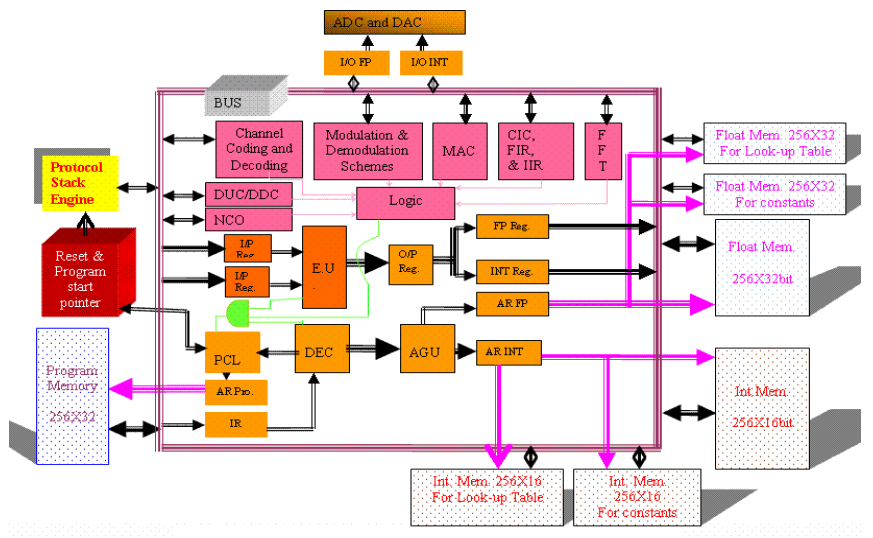
\includegraphics[scale=0.61]{arch.png}
  \caption{Proposed architecture for SDR by Raju, Shekhar, 
           and Joshi \cite{arch}.}
\end{center}
\end{figure}

\item \textbf{Implementation of Cognitive Engine}: This involves designing a 
solution for dynamic spectrum sharing problem. The engine shall sense the 
spectrum and decide which channels will be used in an intelligent manner. 
By `decision', we mean that CE will execute the appropriate instructions on 
the SDR processor to perform the task that the CE specifies.

\begin{figure}[H]
\begin{center}
  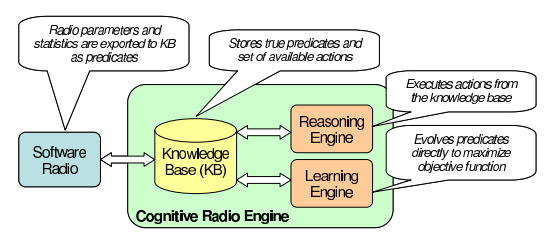
\includegraphics[scale=0.75]{engine.png}
  \caption{Cognitive Engine role. \cite{planning}.}
\end{center}
\end{figure}

\end{enumerate}

\section{Etymology}

The title of the project is inspired by the naming of ``Radio K.A.O.S''
studio album by Roger Waters, former Pink Floyd member \cite{kaos}.

\begin{figure}[H]
\begin{center}
  
\includegraphics[scale=0.2]{kaos.jpg}
  \caption{Radio KAOS.}
\end{center}
\end{figure}

\begin{thebibliography}{9}
\bibitem{planning}
T. Charles Clancy,
Zhu Ji,
Beibei Wang,
K. J. Ray Liu.
``\textit{Planning Approach to Dynamic Spectrum Access
in Cognitive Radio Networks}''.

\bibitem{dynamic}
Usama Mir,
Leila Merghem-Boulahia,
Moez Esseghir,
D. Gaiti.
``\textit{Dynamic spectrum sharing for cognitive radio networks 
using multiagent system}'' in IEEE Consumer Communications and 
Networking Conference, Jan 2011.

\bibitem{arch}
K. Solomon Raju, Chandra Shekhar, R C Joshi.
``\textit{Design of an architecture and instruction set of a
reconfigurable ASIP for Software-Defined Radio}''.

\bibitem{kaos}
``\textit{The Story Of Radio K.A.O.S.}'' Retrieved from
\url{http://www.rogerwaters.org/kaos.html}.

\end{thebibliography}

\end{document}
